\clearpage
\section{Test Results - White Box Testing}
In this section we have explored the source code from the Amu-Darya website. Unfortunately, we did not manage to set up the server locally on our computer. Because of this, it was hard to do any testing in debug mode. To test the source code we have used a few tools as well as reading through the source code manually. Our test plan mainly focused on sections from the OWASP Top 10 Source Code Flaws and will be our foundation for the results.

\subsection{Poor Input Validation}
We did a scan with the CDG code analyzer tool, which returned a summary of potential safety holes in the source code. The summary exposed a lot of poor input validation; input submitted by forms is apparently not being sanitized properly, which allows attacks like cross-site scripting and SQL injection.

\subsubsection{Cross-Site Scripting}
XSS is not validated at all. All input fields and GET-parameters are prone to exploitation.

\begin{lstlisting}
<form action="registerCustomer.do" method="post">
                                    <input id="email" name="email" type="text" />
                                	<input id="name" name="name" type="text" />
<input id="password" name="password" type="text" autocomplete="off" />
                        	<input type="submit" value="Submit">
</form>
\end{lstlisting}
{\em Above: A form for filling in email-address, name and password when registering a new user. No data validation. Only "security measure" found is "autocomplete=off" in password. User is free to inject code.}


\subsubsection{SQL Injection}
Most of the database queries (updates and inserts) use "prepared statement". This prevents malicious code being executed in the database, as the input is saved as a string. However, this is not done throughout the application, and queries such as "find a book by ISBN", "Register new customer", "Find customer by mail" and "Activate customer", enables a user to input code that could potentially alter the database, and/or send more information to the user than originally intended.

\begin{lstlisting}
String query = "INSERT INTO customer (email, password, name, activation_token) VALUES ('"
                    + customer.getEmail()
                	+ "', '"
                	+ customer.getPassword()
                	+ "', '"
                	+ customer.getName()
                	+ "', '"
                	+ customer.getActivationToken()
                	+ "')";
        	statement.executeUpdate(query);
\end{lstlisting}
{\em Above is an extraction from the source code, where the registration of a new customer takes place. A user is able to directly write SQL-code instead of, for instance, the user's email-address.}

\begin{lstlisting}
String query = "UPDATE customer SET email=?, password=?, name=? WHERE id=?";
            statement = connection.prepareStatement(query);
        	statement.setString(1, customer.getEmail());
        	statement.setString(2, customer.getPassword());
        	statement.setString(3, customer.getName());
        	statement.setInt(4, customer.getId());
\end{lstlisting}
{\em Above is an extraction from the source code, where an update on an existing customer takes place. The system "prepares" the code} before {\em executing it with the input.}

We attempted to do SQL injections during black box testing, but we did not manage to do much without information considering the structure of a query. Using the source code as a reference, we found additional places for injection opportunities. From the application's point of view, it is possible to run extra updates or other statements at certain places specified above, but every time we tried to execute them, the server returned the error message: {\em The full stack traces of the exception}.

\subsection{Database Vulnerabilities}
It is great that the passwords are encrypted, but this is not the only information that should be encrypted. Sensitive information about a user (customer) should also be protected. In the database, credit card information is stored in plain text. Should the database be breached by someone, the credit card information should not be this easily obtainable.

\subsection{Hardcoded Values}
In the config file we found the hardcoded values for the email password ((EMAIL\textunderscore SMTP\textunderscore PASSWORD)) and the salt for the hashing algorithm. The same salt is used for all user accounts.

\begin{lstlisting}
public final static String SALT="NaCl"; // Changing this will invalidate all customer passwords in DB
\end{lstlisting}
{\em Above: Hardcoded salt from Config.java file.}

This is a security risk, as the purpose of having a salt is to make it more difficult for someone to regenerate the password hashcode; the salt should be randomly generated for each individual user, and should certainly not be hardcoded in the source code. Knowing salt and hashing algorithm (the {\em SHA-1 algorithm}, as previously assumed in the black box testing results) makes it easier to encrypt the password using Rainbow tables. Simply having one, never-changing salt for all users does not increase the time used in cracking passwords (when the correct set of possible symbols and password length are found). It is possible to generate a user with an empty password. In this case the salt itself is the only hash stored in the database for this user, and by using CrackStation, or similar software/webpages, we were able to decrypt the salt.

\begin{figure}[!ht]
  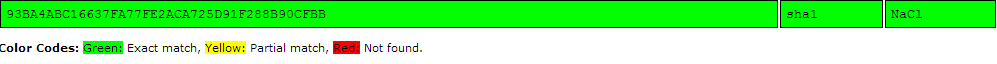
\includegraphics[scale=0.5]{pics/tre.png}
\end{figure}

Previously when creating rainbow chains we made a mistake in selecting charset. We used lower-alpha assuming that just for test purpose the password will only contain small letters. Now we know that we should use mixalpha to include both small and big letters. It takes long time to create Rainbow chains, but they crack the password with 99 \% probability and it only takes a few seconds to convert the hashcode to plaintext. Below you will find a result from our test, where we cracked small passwords for test purpose, to reduce the time for creating chains.

\begin{figure}[!ht]
  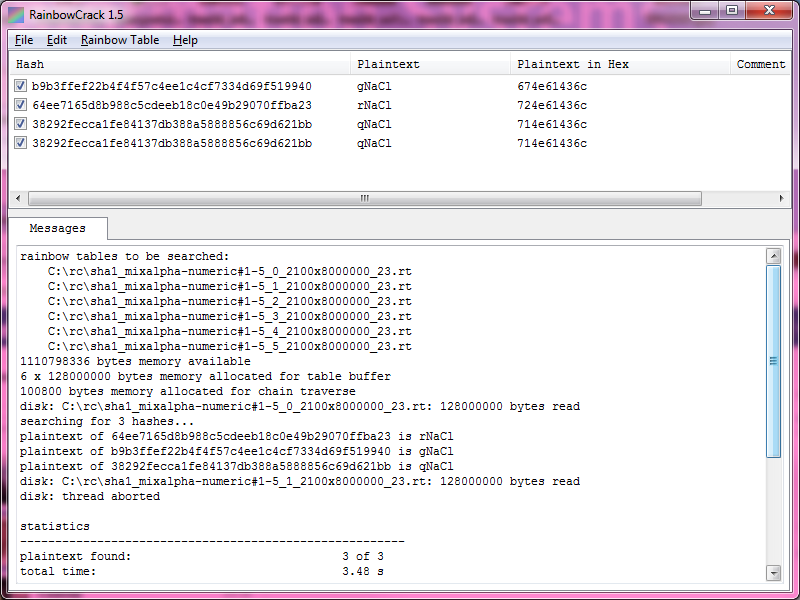
\includegraphics[scale=0.8]{pics/Untitled.png}
\end{figure}


\subsection{Session Handling, Cookies and Communication}
The system uses the Java API for session handling, and the sessionID is generatedby standard Java function. However, the cookie content is not encrypted, and could be a vulnerability (mentioned in black box test results).


\subsection{Potentially Dangerous APIs/Auxiliary Systems}
The application does not appear to be using any third-party APIs. Neither does it seem to use any deprecated methods from the Java API, nor is it overly-dependent on any auxiliary systems.
